温度$T_b=0$℃、一定の無限平板(厚さ 20 \si{\cm})の片側表面を急に$T_a = 1000$℃にした場合の温度変化に関して、
前進差分法のトーマス法による数値解析をソースコード\ref{s1}に示す。時間ステップは250 \si{s}、解析結果を1000 \si{s}ごとに5000 \si{s}
ごとに出力したものを図\ref{im1}に示す。
\begin{lstlisting}[caption=前進差分法のトーマス法による数値解析プログラム,label=s1]
#include <stdio.h>

#define N 10            // メッシュ数
#define L 0.2           // 棒の長さ
#define dx (L / N)      // メッシュの間隔
#define T0 1000.0       // 左端の温度
#define T1 0.0          // 右端の温度
int T_FINAL = 5000;     // 解析終了時間
#define a (1.26/(1600*1050))// 熱伝達率
#define dt 250          // 時間刻み幅
  
int main()
{
  double T[N+1];      // 未知数の温度分布
  double T_new[N+1];  // 次の時間ステップの温度分布

  // 初期条件の設定
  for (int i = 0; i < N+1; i++) {
    T[i] = 0.0;     // 初期温度分布を0℃で初期化
  }

  // 時間ステップごとの反復
  int t = 0;
  double r = a*dt/(dx*dx);
  while (t <= T_FINAL) {
    T[0] = T0;      // 左端の境界条件
    T[N+1] = T1;    // 右端の境界条件
    // トーマス法による解の計算
    for (int i = 1; i < N; i++) {
      double k_1 = r;
      double k_2 = 1 - 2 * r;
      T_new[i] = k_1 * T[i - 1] + k_2 * T[i] + k_1 * T[i + 1];
    }
  
    // 結果の出力
    if(t % 1000 == 0 && t != 0){
      printf("%d[s] ",t);
      for(int i = 0; i < N+1; i++){
        printf("%5.1f\t",T[i]);
      }
      printf("\n");
    }
    // 次の時間ステップの温度分布を更新
    for (int i = 1; i < N; i++) {
      T[i] = T_new[i];
    }
    t += dt; // 時間を進める
  }
  return 0;
}
\end{lstlisting}

\begin{figure}[H]
  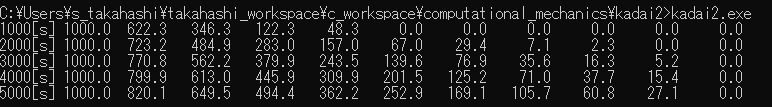
\includegraphics[width=\columnwidth]{img/k2.png}
  \caption{実行結果}
  \label{im1}
\end{figure}